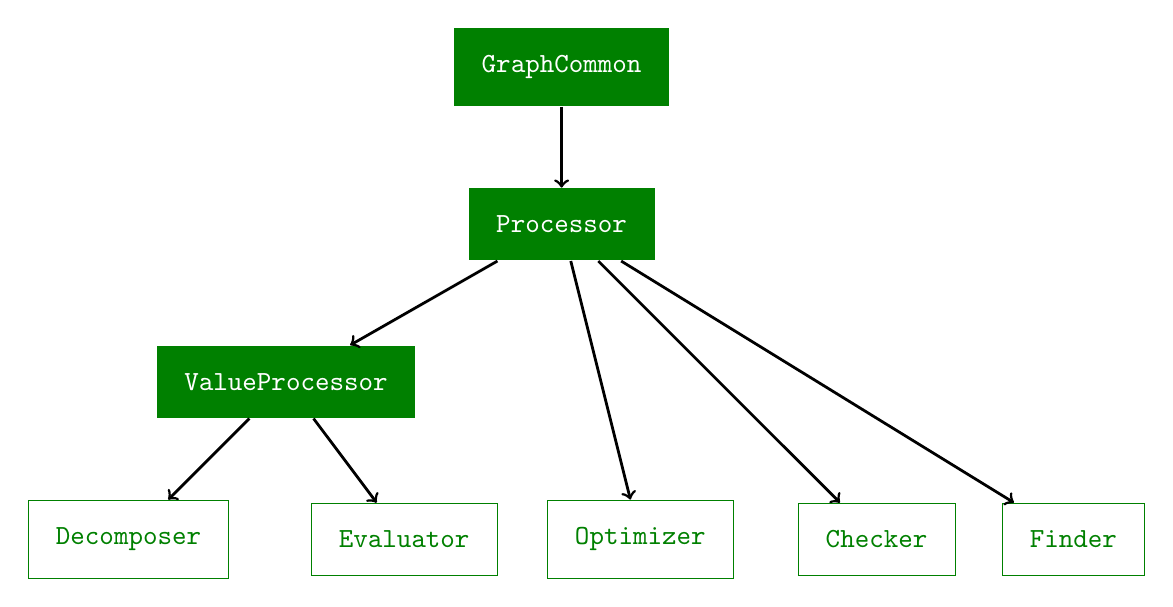
\begin{tikzpicture}
\tikzstyle{class} = [font=\ttfamily\bfseries,color=white,fill=green!50!black,inner sep=10];
\tikzstyle{struct} = [font=\ttfamily\bfseries,color=blue,draw=blue, inner sep = 5];
\tikzstyle{member} = [font=\ttfamily,draw, inner sep=5]
\tikzstyle{function} = [font=\ttfamily\bfseries,color=red,draw=red, inner sep = 5];
\tikzstyle{subclass} = [font=\ttfamily\bfseries,color=green!50!black,draw=green!50!black,inner sep=10];
\tikzstyle{arr} = [line width=1,->];
\node [class] (v1) at (1.5,4) {GraphCommon};
\node [class] (v2) at (1.5,2) {Processor};
\node [class] (v3) at (-2,0) {ValueProcessor};
\node [subclass] (v4) at (-4,-2) {Decomposer};
\node [subclass] (v5) at (-0.5,-2) {Evaluator};
\node [subclass] (v6) at (2.5,-2) {Optimizer};
\node [subclass] (v7) at (5.5,-2) {Checker};

\node [subclass] (v8) at (8,-2) {Finder};
\draw[arr]  (v1) edge (v2);
\draw [arr] (v2) edge (v3);
\draw [arr] (v3) edge (v4);
\draw [arr] (v3) edge (v5);
\draw [arr] (v2) edge (v6);
\draw [arr] (v2) edge (v7);
\draw [arr] (v2) edge (v8);
\end{tikzpicture}